\chapter{Extending surface hopping}
\label{chap:surface_hopping_ES}

\noindent FOB-SH is a variant of Tully's original fewest switches surface hopping \cite{FSSH_orig}. It has been used to simulate electron-nuclear dynamics in large systems of organic molecules and has been well tested against experimental studies and benchmarked against higher order studies \cite{FlickPolarons, Giannini2018Crossover, Giannini2019,             C9TC05270D, Carof2017FSSH, C9FD00046A, C9CP04770K, FOB-SH_Spencer,        C6FD00107F}. However, the code does not currently account for any electrostatic interactions. This presents a problem when looking at many systems; such as those with large amounts of disorder or those with polariseable molecules. 
%Need more motivation of implementing electrostatics in CP2K
\\\\
The standard Coulomb sum of partial charges is only conditionally convergent and extremely slow to calculate. The standard method for calculating electrostatic interactions is by decomposing interactions into long-range and short-range interactions (with corrections such as removing bonded terms etc\ldots). This is normally carried out with an Ewald sum \cite{Ewald} where a short-range interactions are calculated in real space and long-range interactions are calculated in reciprocal space. This results in 2 summations that are now unconditionally, quickly convergent. Further extensions to the standard Ewald technique provide an additional decrease in computational time by interpolating particles onto a grid and using fast fourier transforms to calculate the sums. In Wolf, 99 \cite{Wolf99}, a technique for removing the (expensive) reciprocal space term from the sum altogether was proposed by ensuring charge neutrality within a cutoff sphere from each atom. This idea was developed to improve energy conservation and to remove discontinuities within the forces and energies \cite{Zahn2002, DSF}. In this work I will investigate the applicability of both the standard Ewald technique and a development of the Wolf method (named DSF \cite{DSF}) to calculate the electrostatic interactions within FOB-SH.
\section{Implementation details}
\subsection{Addition Subtraction Method}
\begin{figure}[ht]
  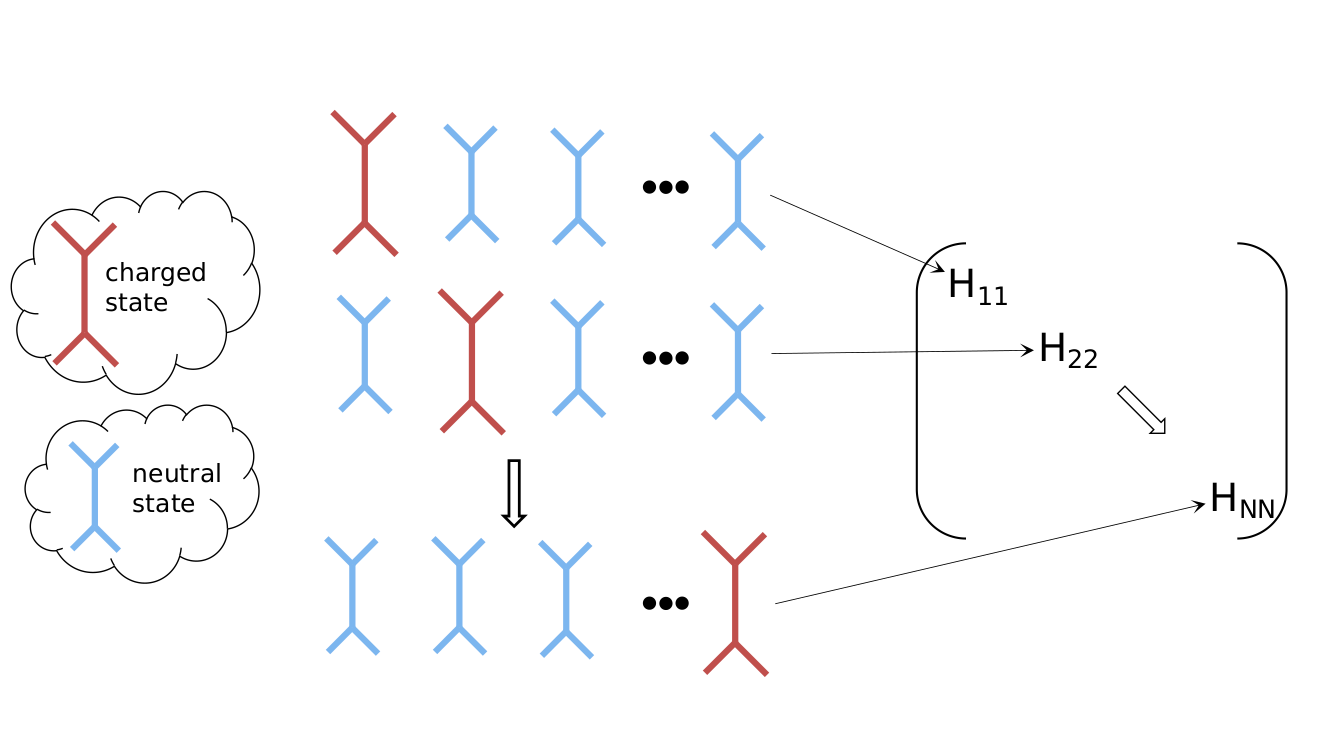
\includegraphics[width=\textwidth]{./img/ES/ForceEnerCalc.png}
  \caption{\label{fig:FE_Calc}A demonstration of the procedure to calculate diagonal elements of the Hamiltonian (site-energies). Red (blue) shapes represent a molecule in it's charged (neutral) state. A  horizontal line of these shapes represent the full system with all molecules; where a single molecule is in it's charged state. The arrow denotes which matrix element this saved as.}
\end{figure}
\noindent In FOB-SH, nuclear dynamics are determined by the Hamiltonian. The Hamiltonian is constructed such that the diagonal elements (site-energies) come from a classical forcefield and the off-diagonal elements (electron couplings) are proportional to the overlap of the diabatic wavefunctions. Each site-energy, $H_{\gamma \gamma}$, is defined as the potential energy of the system where the excess charge is localised on the molecule $\gamma$. For the avoidance of doubt, I will denote the molecule with the excess charge localised on it as the `charged' molecule and other molecules as `neutral'. The presence of the excess charge on molecule $\gamma$ results in different input parameters (such as the charge distribution or the length of bonds) than the other neutral molecules. This results in the calculation of site-energies and forces having to be repeated $N_{mol}$ times for each permutation of the charged molecule. This is summarised in figure \ref{fig:FE_Calc}. 
\\\\
To determine whether it is feasible to repeat the calculation of the electrostatic interactions $N_{mol}$ times a quick timing run was carried out. This simulated 250 pentacene molecules (9,000 atoms) and the time was measured to calculate the electrostatic interactions with the 3 methods already implemented within CP2K: Smooth Particle Mesh Ewald (SPME), Particle Mesh Ewald (PME) and standard Ewald. The measured time of a simulation without any electrostatics was then subtracted from each of these simulations to isolate the time spent on just the electrostatics. The results are given in figure  \ref{fig:ES_Timings}.
\begin{figure}[ht]
  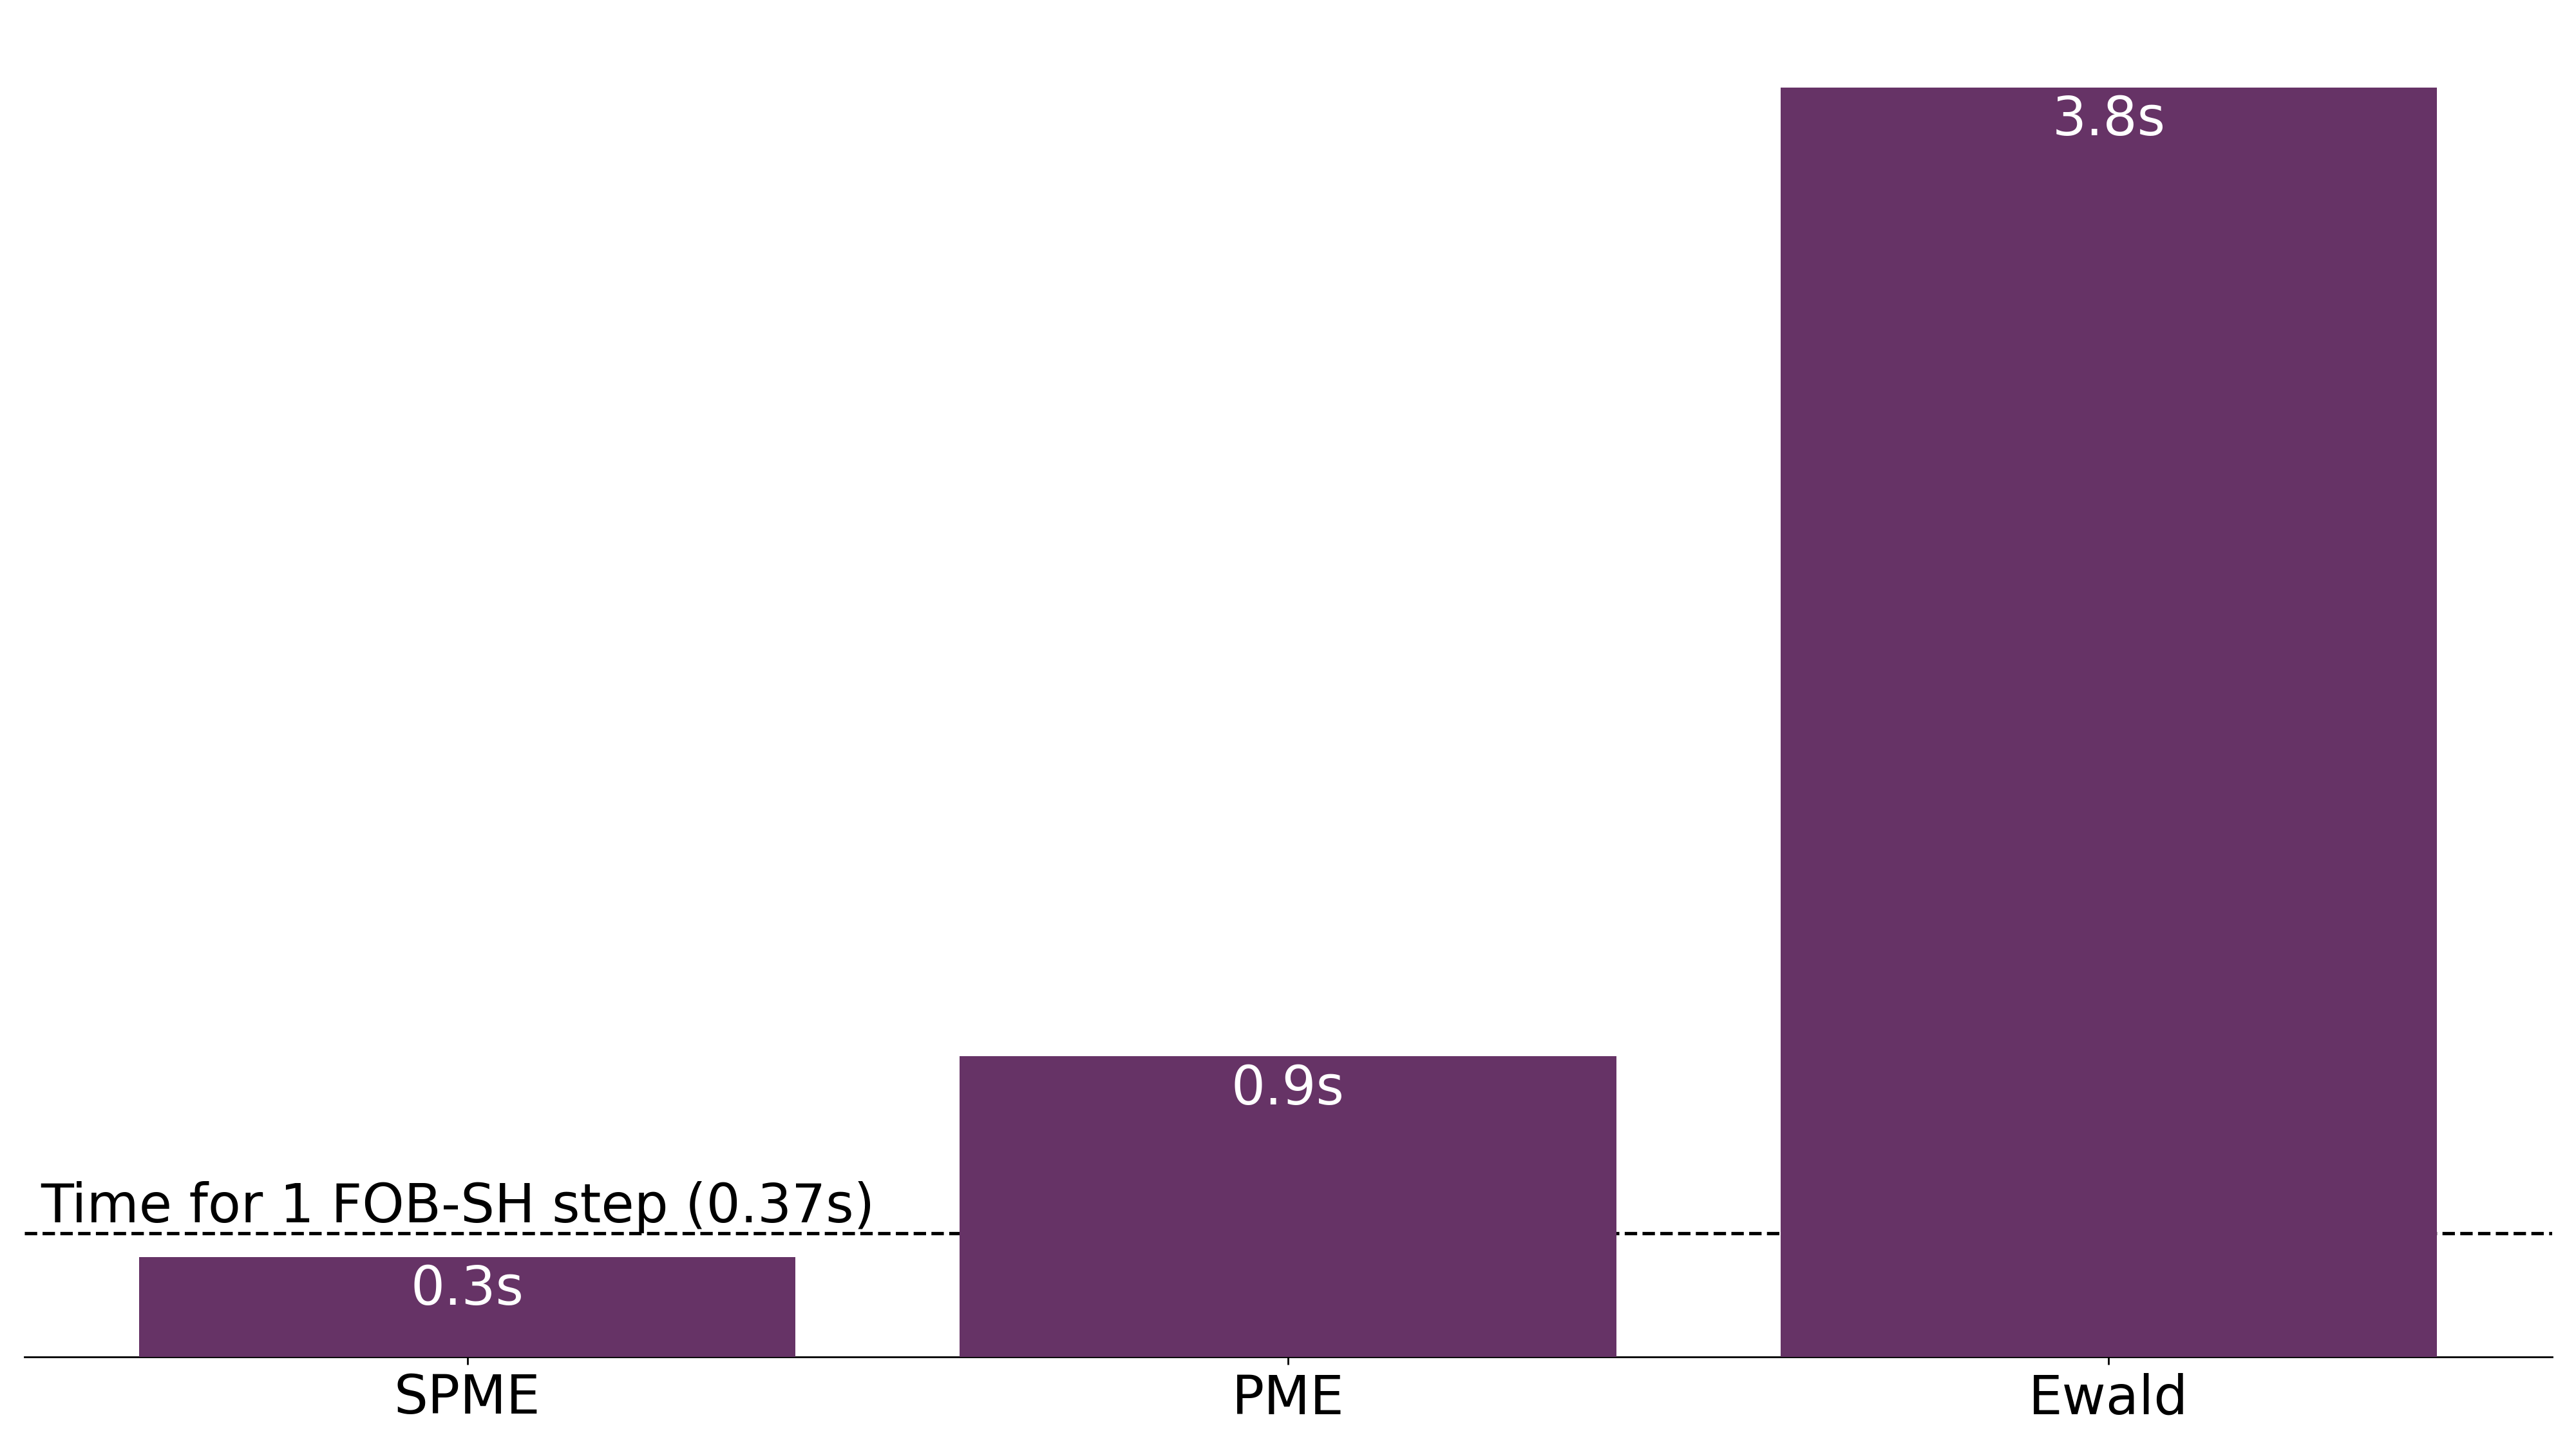
\includegraphics[width=\textwidth]{./img/ES/InitialTimings.png}
  \caption{\label{fig:ES_Timings}The time taken to calculate just the electrostatic interactions within CP2K for a 9,000 atom system using various methods. PME is particle mesh Ewald, SPME is smooth-PME, Ewald is the standard ewald method. The dashed line shows the time taken for a single FOB-SH step.}
\end{figure}
\\
We can see that even a single calculation of the electrostatic interactions with the fastest method available within CP2K will take a comparable time to the rest of the surface hopping code. It is clear then that a more efficient method must be used to calculate the electrostatics in a more efficient way.
\\
\begin{figure}[ht]
  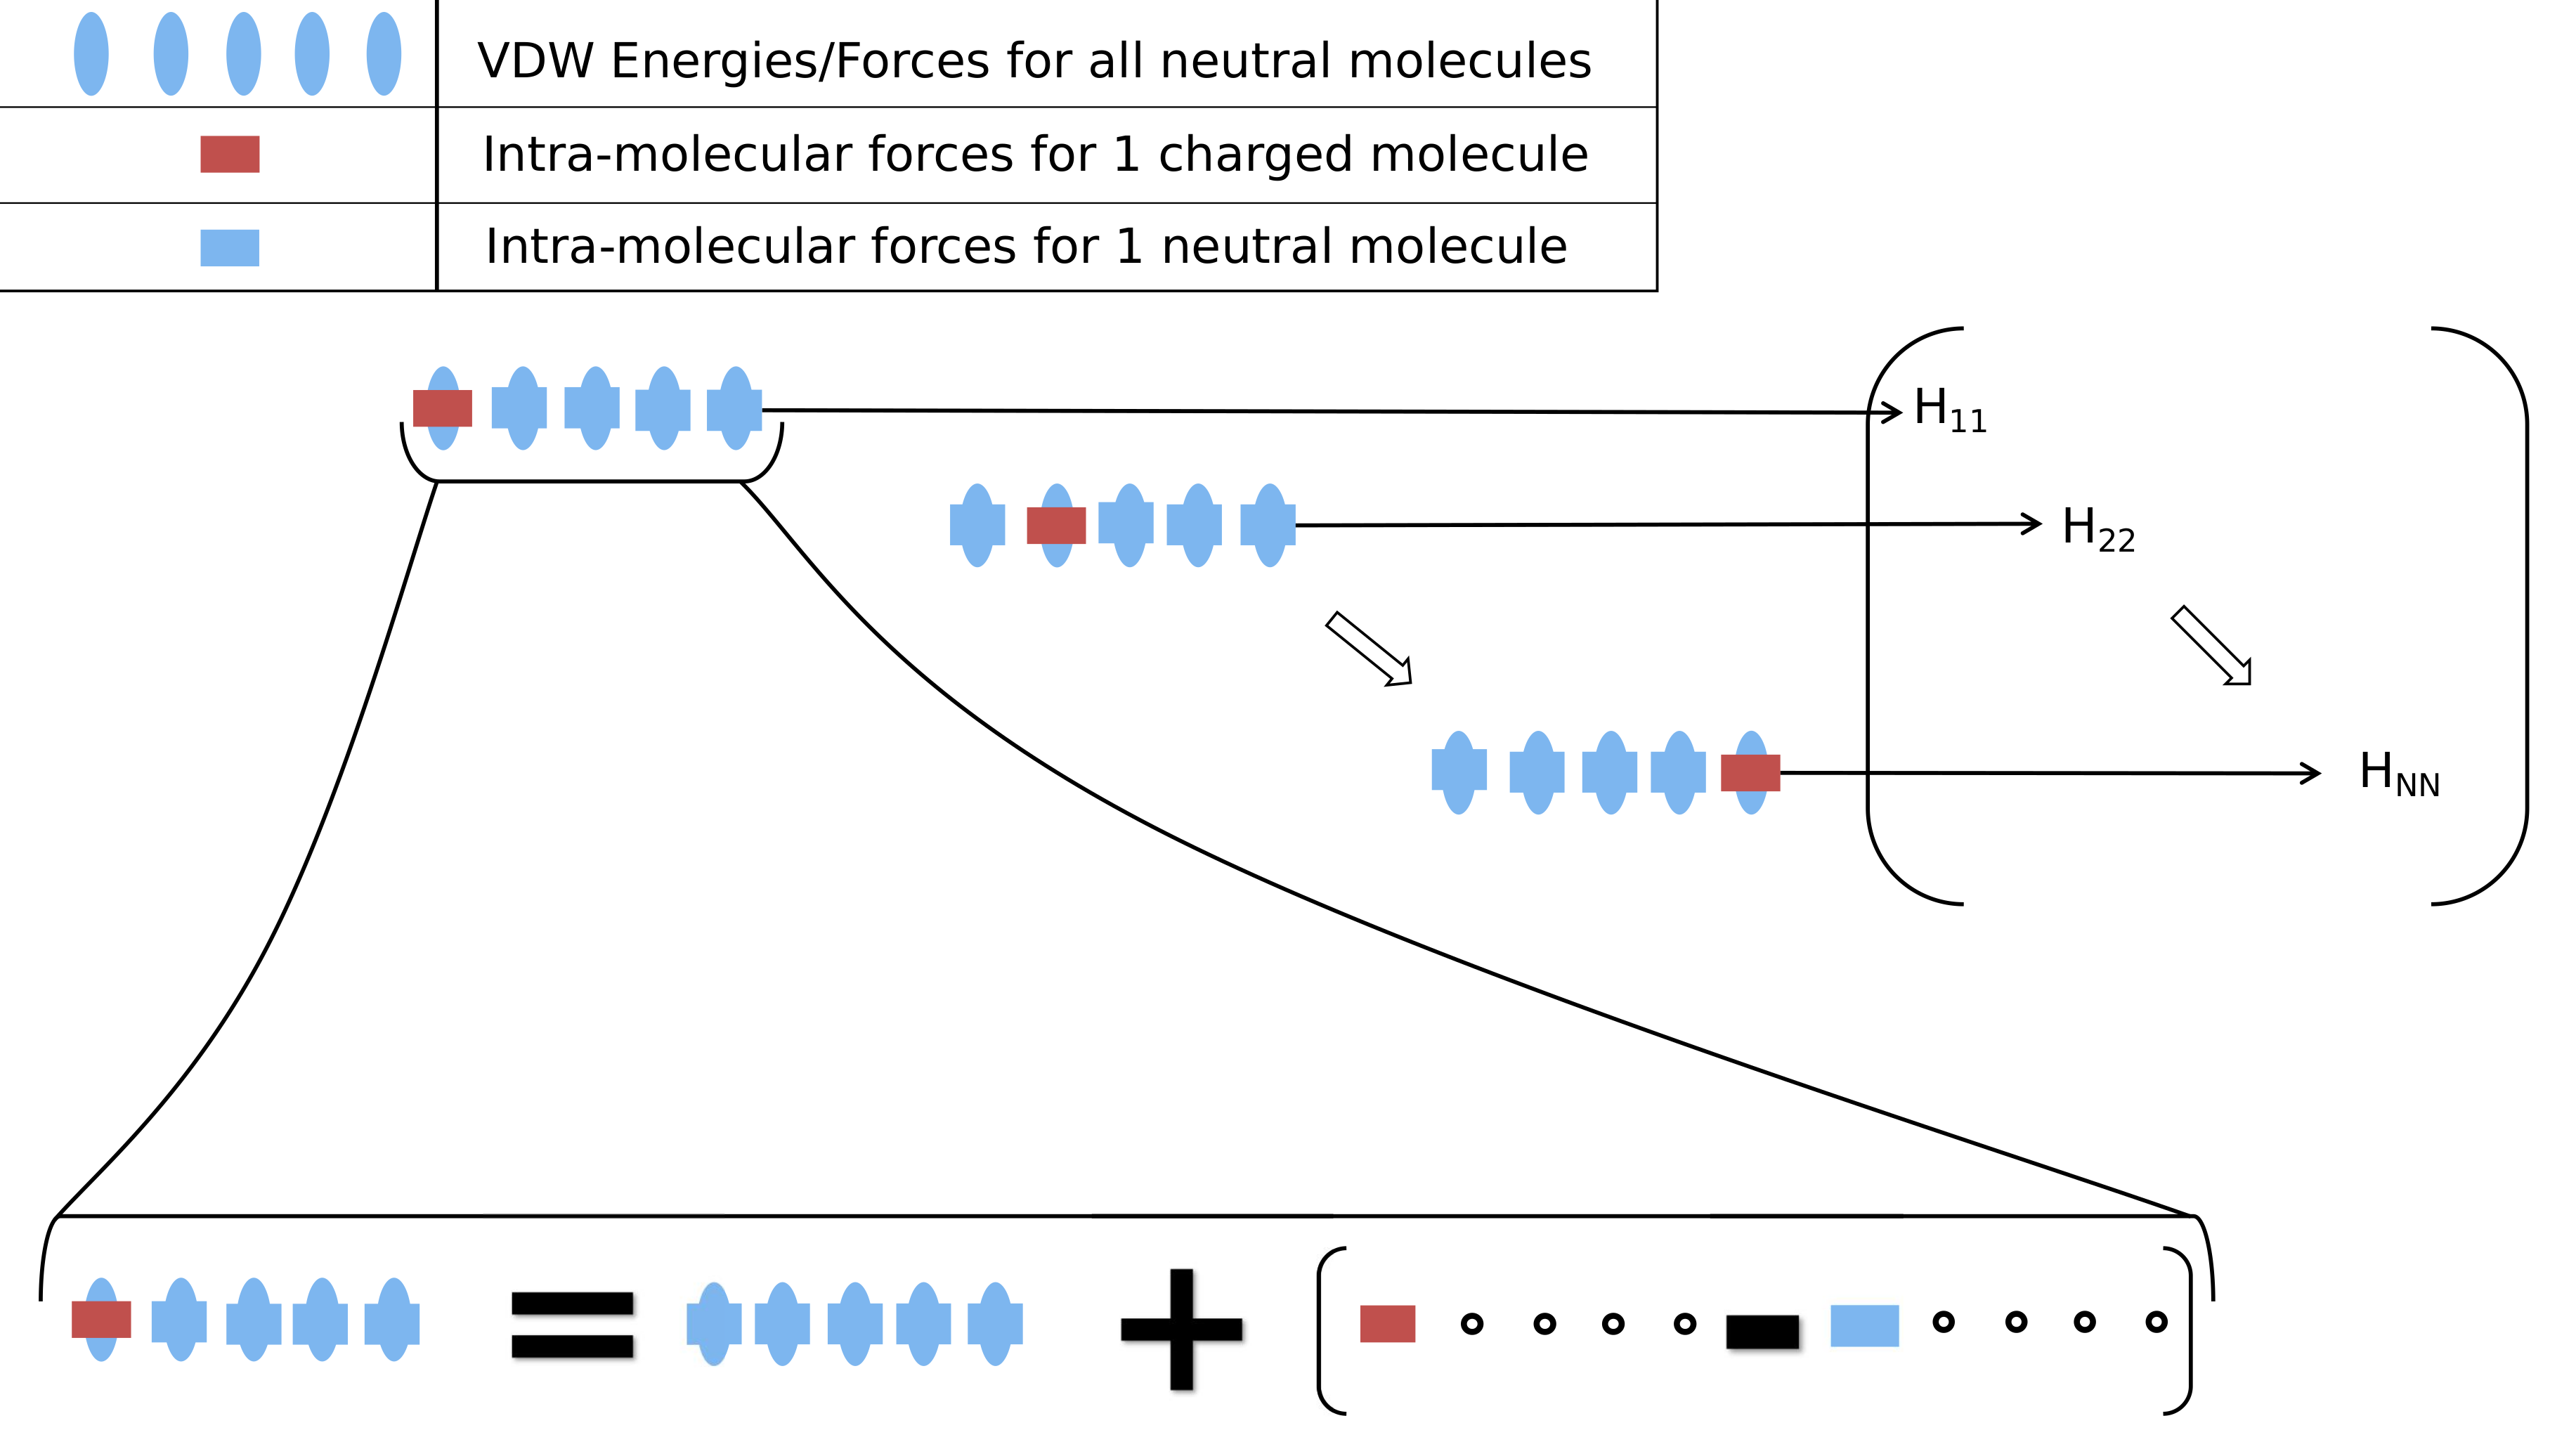
\includegraphics[width=\textwidth]{./img/ES/ForceEnerDecomp.png}
  \caption{\label{fig:enerF_decomp}A depiction of the decomposition of the forces and energies within FOB-SH. First the all neutral VDW forces/energies are computed (blue ovals). Second the intra-molecular forces for each charged (neutral) molecule, represented by a red (blue) rectangle. The site-energy/force is then computed as a summation of all molecules in their neutral state with a molecule in its neutral state subtracted and the same molecule in its charged state added.} 
\end{figure}
\\
Within the current FOB-SH implementation the forces and energies consist of intra-molecular components (bonds, bends, torsions etc\ldots) and inter-molecular components (Van der Waals forces provided by a Leonard-Jones potential). The same repetition of the calculation of forces and energies would, at first glance, be required for the correct calculation of these terms. However, an addition-subtraction scheme is used to reduce the calculation time from $O(N_{mol}, N_{atom}^2)$ to $O(N_{atom}^2)$. This is summarised in figure \ref{fig:enerF_decomp} and relies on the fact that the intra-molecular forces and energies can be decomposed into independent molecular contributions. In order to calculate the force on each atom and site-energy with molecule $\gamma$ in its charged state the code first calculates the force/energy with all molecules in their neutral state and then adds the contribution of molecule $\gamma$ in its charged state and subtracts the contribution of molecule $\gamma$ in its neutral state. We do not make the same adjustment for the VDW forces as the correction is negligible. This results in just 2 calculations of all forces and total energies rather than $O(N_{mol})$ calculations. Seeing as the electrostatics are normally one of the most expensive parts of a classical force-field it is particularly important that these are treated efficiently.
\\\\
The addition subtraction scheme applied to the electrostatic interactions cannot be the same as the one used for the intra-molecular interactions as separate molecules are not independent and energies and forces cannot be decomposed into molecular contributions for each different site-energy. However, a similar trick can be used, though this can only be applied to the real-space component of the Ewald sum.
\subsection{Ewald Equations and the additional subtraction scheme}
The standard Ewald summation for evaluating electrostatic energies in molecular dynamics simulation are given below:
\begin{eqnarray}
E_{coul}\left(\mathbf{r}^{N}\right)
=
% Real Space Sum
 \frac{1}{4 \pi \epsilon_0} \sum_{j}^{N_{at}} \sum_{i > j}^{N_{at}} q_i q_j \frac{erfc\left( \alpha \cdot |\mathbf{r}_{ij}|\right)}{|\mathbf{r}_{ij}|} \Theta\left( r_{cut} - |\mathbf{r}_{ij}| \right)
\\
% Reciprocal Space Sum
+
\frac{1}{2\pi V} \ \frac{1}{4 \pi \epsilon_0} \sum_{\mathbf{k} \neq 0} \frac{1}{|\mathbf{k}|^2} e^{-\frac{\pi^2 \ |\mathbf{k}|^2}{\alpha^2}} \ \left|\sum_{j}^{N} q_{j} e^{2\pi i \mathbf{k} \cdot \mathbf{R}_{j}}\right|^2 \\
% Self Term
- \frac{\alpha}{\sqrt{\pi}} \frac{1}{4 \pi \epsilon_{0}} \sum_{j} q_{j}^2
\\
- \text{ \ other corrections such as dipole etc...}
\label{eq:EwaldStd}
\end{eqnarray}




